\documentclass[12pt, twoside]{article}
\usepackage[francais]{babel}
\usepackage[T1]{fontenc}
\usepackage[latin1]{inputenc}
\usepackage[left=5mm, right=5mm, top=3mm, bottom=3mm]{geometry}
\usepackage{float}
\usepackage{graphicx}
\usepackage{array}
\usepackage{multirow}
\usepackage{amsmath,amssymb,mathrsfs}
\usepackage{soul}
\usepackage{textcomp}
\usepackage{eurosym}
 \usepackage{variations}
\usepackage{tabvar}

\pagestyle{empty}

\begin{document}

\begin{flushleft}
NOM PRENOM: \ldots \ldots \ldots \ldots \ldots \ldots \ldots \ldots \ldots
 
\enskip

\end{flushleft}

\begin{center}
{\fbox{$3^{e}2$ \qquad \qquad \textbf{\Large{Mini-test 13 (sujet 1)}}
\qquad \qquad 29/05/2013}}
\end{center}



\enskip 


\ul{Exercice 1}: \textit{3 points}

Dire si les fonctions ci-dessous sont affines ou non.

\begin{center}
 $f(x)=-9x^2-3$ \ldots \ldots \qquad \qquad 
 \quad $g(x)=\dfrac{3}{4}-\dfrac{2}{x}$ \ldots \ldots \qquad \qquad \quad 
 $h(x)=12-2x$ \ldots \ldots
 \end{center}


\bigskip

\ul{Exercice 2}: \textit{4 points}

On consid�re la fonction affine $k: x \mapsto 5-2x$.

\begin{enumerate}
  \item Donner l'image de -7 par la fonction $k$. \quad \ldots \ldots \ldots
  \ldots \ldots \ldots \ldots \ldots \ldots \ldots \ldots \ldots \ldots \ldots
  \ldots \ldots \ldots \ldots
  \item Donner l'ant�c�dent de 4 par la fonction $k$. \quad \ldots \ldots \ldots
  \ldots \ldots \ldots \ldots \ldots  \ldots \ldots \ldots \ldots \ldots \ldots
  \ldots \ldots \ldots 
  \item Donner le coefficient directeur de la fonction $k$. \quad \ldots \ldots
  \ldots \ldots \ldots \ldots \ldots \ldots  \ldots \ldots \ldots \ldots \ldots
  \ldots \ldots \ldots 
  \item Donner l'ordonn�e � l'origine de la fonction $k$. \quad \ldots \ldots
  \ldots \ldots \ldots \ldots \ldots \ldots  \ldots \ldots \ldots \ldots \ldots
  \ldots \ldots \ldots 
\end{enumerate}

\bigskip

\ul{Exercice 3}: \textit{5 points}

\begin{tabular}{cc}
\begin{minipage}{5cm}
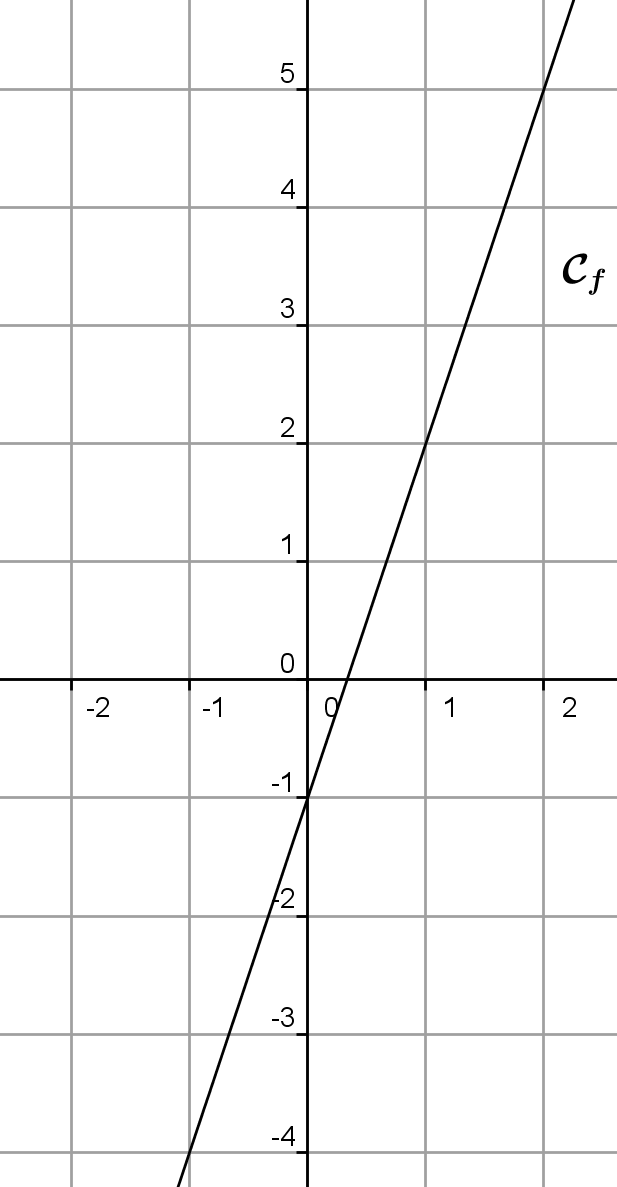
\includegraphics[width=3cm]{images/ex3-1.png} 
\end{minipage}
&
\begin{minipage}{14cm}

On consid�re la repr�sentation graphique de la fonction $f$. 

\enskip

Vous laisserez tous
vos traits de construction apparents.


\begin{enumerate}
  \item Donner l'image de -1 par la fonction $f$? \qquad \ldots \ldots
  \ldots \ldots \ldots
  \item Lire l'ant�c�dent de 2 par la fonction $f$. \qquad \ldots \ldots \ldots
  \ldots \ldots
  \item Quelle est l'ordonn�e � l'origine de la fonction $f$? \qquad \ldots \ldots \ldots
   \ldots \ldots
  \item Quel est le coefficient directeur de la fonction $f$? \qquad \ldots \ldots \ldots
   \ldots \ldots  
   \item Donner l'expression alg�brique de la fonction $f$. \qquad \ldots
   \ldots \ldots \ldots \ldots  
\end{enumerate}
\end{minipage}
\end{tabular}

\bigskip

\ul{Exercice 4}: \textit{3 points}


\begin{tabular}{cc}
\begin{minipage}{10cm}
Soit $g: x  \mapsto -3x+2$.

\enskip

Tracer la repr�sentation graphique de $g$ (vous �crirez vos calculs ou
laisserez vos traits de construction apparents).

\bigskip

\bigskip

\bigskip

\bigskip

\bigskip

\bigskip

\bigskip

\bigskip

\end{minipage}
& 

\begin{minipage}{8cm}
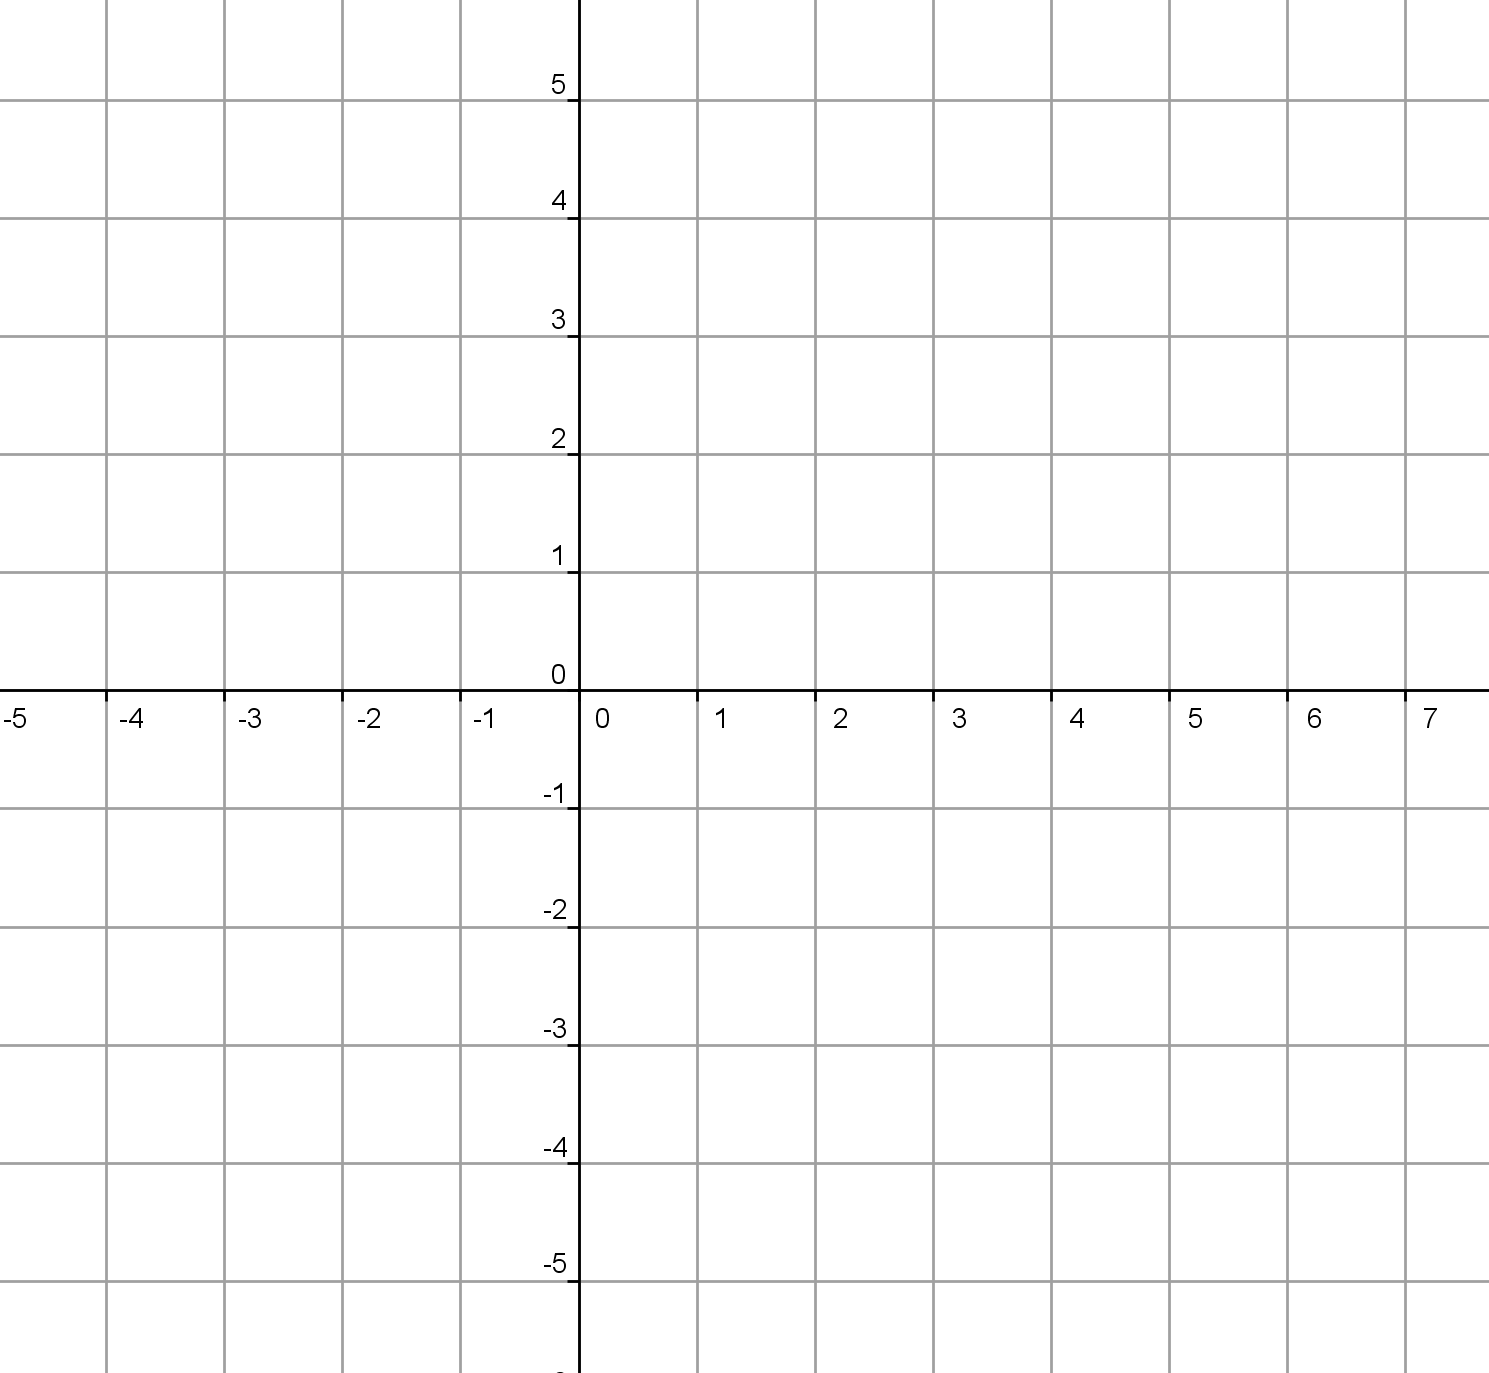
\includegraphics[width=7cm]{images/ex4.png} 
\end{minipage}
\end{tabular}

\bigskip

\ul{Exercice 5}: \textit{5 points}

Soit une fonction affine $k$.
Les points D(3;4) et E(-7;2) appartiennent �  sa repr�sentation graphique.

\begin{enumerate}
  \item Calculer le coefficient directeur de la fonction $k$.
  \item Calculer l'ordonn�e � l'origine de la fonction $k$.
  \item Donner l'expression alg�brique de la fonction $k$.
\end{enumerate}


\ldots \ldots \ldots \ldots \ldots \ldots \ldots \ldots \ldots \ldots \ldots
\ldots \ldots \ldots \ldots \ldots \ldots \ldots \ldots \ldots \ldots \ldots
\ldots \ldots \ldots \ldots \ldots \ldots \ldots \ldots \ldots \ldots \ldots
\ldots \ldots \ldots  

\ldots \ldots \ldots \ldots \ldots \ldots \ldots \ldots \ldots \ldots \ldots
\ldots \ldots \ldots \ldots \ldots \ldots \ldots \ldots \ldots \ldots \ldots
\ldots \ldots \ldots \ldots \ldots \ldots \ldots \ldots \ldots \ldots \ldots
\ldots \ldots \ldots  

\ldots \ldots \ldots \ldots \ldots \ldots \ldots \ldots \ldots \ldots \ldots
\ldots \ldots \ldots \ldots \ldots \ldots \ldots \ldots \ldots \ldots \ldots
\ldots \ldots \ldots \ldots \ldots \ldots \ldots \ldots \ldots \ldots \ldots
\ldots \ldots \ldots  

\ldots \ldots \ldots \ldots \ldots \ldots \ldots \ldots \ldots \ldots \ldots
\ldots \ldots \ldots \ldots \ldots \ldots \ldots \ldots \ldots \ldots \ldots
\ldots \ldots \ldots \ldots \ldots \ldots \ldots \ldots \ldots \ldots \ldots
\ldots \ldots \ldots  

\pagebreak


\begin{flushleft}
NOM PRENOM: \ldots \ldots \ldots \ldots \ldots \ldots \ldots \ldots \ldots
 
\enskip

\end{flushleft}

\begin{center}
{\fbox{$3^{e}2$ \qquad \qquad \textbf{\Large{Mini-test 13 (sujet 2)}}
\qquad \qquad 29/05/2013}}
\end{center}



\enskip 


\ul{Exercice 1}: \textit{3 points}

Dire si les fonctions ci-dessous sont affines ou non.

\begin{center}
 $f(x)=\dfrac{2}{5}-\dfrac{3}{x}$ \ldots \ldots \qquad \qquad 
 \quad $g(x)=7-4x$ \ldots \ldots \qquad \qquad \quad 
 $h(x)=3x^2+8$ \ldots \ldots
 \end{center}


\bigskip

\ul{Exercice 2}: \textit{4 points}

On consid�re la fonction affine $k: x \mapsto 4-3x$.

\begin{enumerate}
  \item Donner l'image de -2 par la fonction $k$. \quad \ldots \ldots \ldots
  \ldots \ldots \ldots \ldots \ldots \ldots \ldots \ldots \ldots \ldots \ldots
  \ldots \ldots \ldots \ldots
  \item Donner l'ant�c�dent de 6 par la fonction $k$. \quad \ldots \ldots \ldots
  \ldots \ldots \ldots \ldots \ldots  \ldots \ldots \ldots \ldots \ldots \ldots
  \ldots \ldots \ldots 
  \item Donner le coefficient directeur de la fonction $k$. \quad \ldots \ldots
  \ldots \ldots \ldots \ldots \ldots \ldots  \ldots \ldots \ldots \ldots \ldots
  \ldots \ldots \ldots 
  \item Donner l'ordonn�e � l'origine de la fonction $k$. \quad \ldots \ldots
  \ldots \ldots \ldots \ldots \ldots \ldots  \ldots \ldots \ldots \ldots \ldots
  \ldots \ldots \ldots 
\end{enumerate}

\bigskip

\ul{Exercice 3}: \textit{5 points}

\begin{tabular}{cc}
\begin{minipage}{5cm}
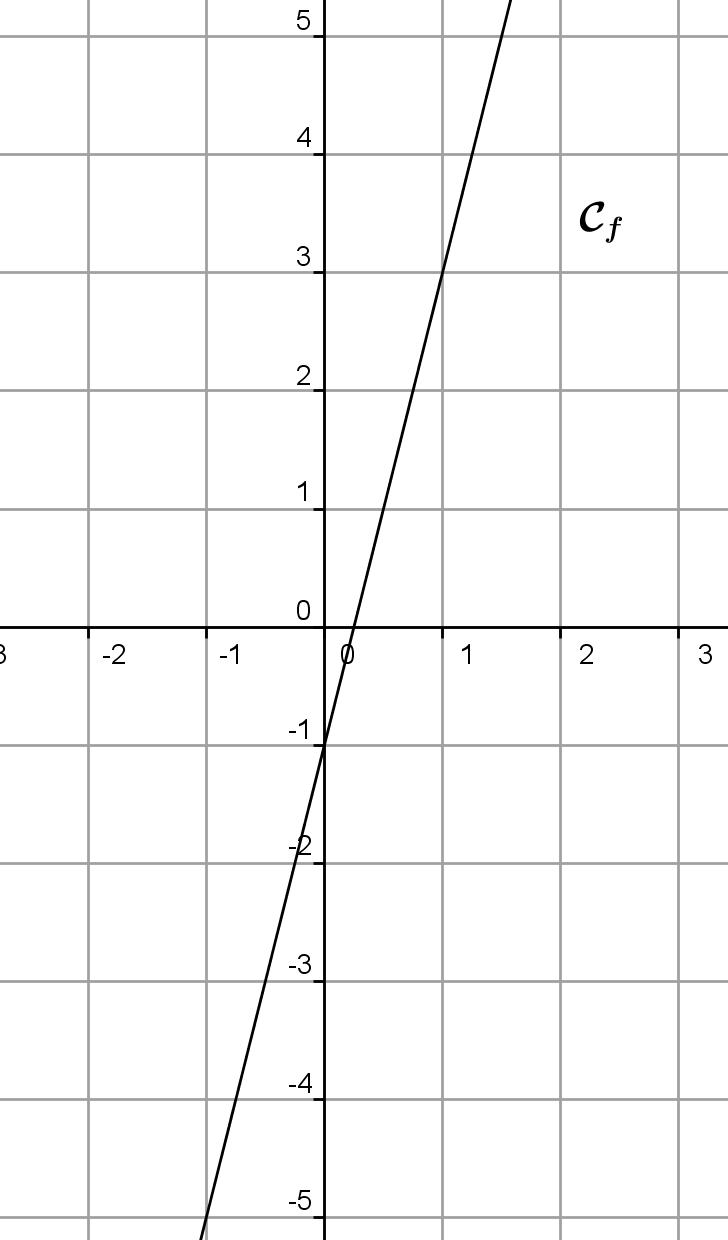
\includegraphics[width=3cm]{images/ex3-2.png} 
\end{minipage}
&
\begin{minipage}{14cm} 

On consid�re la repr�sentation graphique de la fonction $f$. 

\enskip

Vous laisserez tous
vos traits de construction apparents.


\begin{enumerate}
  \item Donner l'image de -1 par la fonction $f$? \qquad \ldots \ldots
  \ldots \ldots \ldots
  \item Lire l'ant�c�dent de 3 par la fonction $f$. \qquad \ldots \ldots \ldots
  \ldots \ldots
  \item Quelle est l'ordonn�e � l'origine de la fonction $f$? \qquad \ldots \ldots \ldots
   \ldots \ldots
  \item Quel est le coefficient directeur de la fonction $f$? \qquad \ldots \ldots \ldots
   \ldots \ldots  
   \item Donner l'expression alg�brique de la fonction $f$. \qquad \ldots
   \ldots \ldots \ldots \ldots  
\end{enumerate}
\end{minipage}
\end{tabular}

\bigskip

\ul{Exercice 4}: \textit{3 points}


\begin{tabular}{cc}
\begin{minipage}{10cm}
Soit $g: x  \mapsto -2x+3$.

\enskip

Tracer la repr�sentation graphique de $g$ (vous �crirez vos calculs ou
laisserez vos traits de construction apparents).

\bigskip

\bigskip

\bigskip

\bigskip

\bigskip

\bigskip

\bigskip

\bigskip

\end{minipage}
& 

\begin{minipage}{8cm}
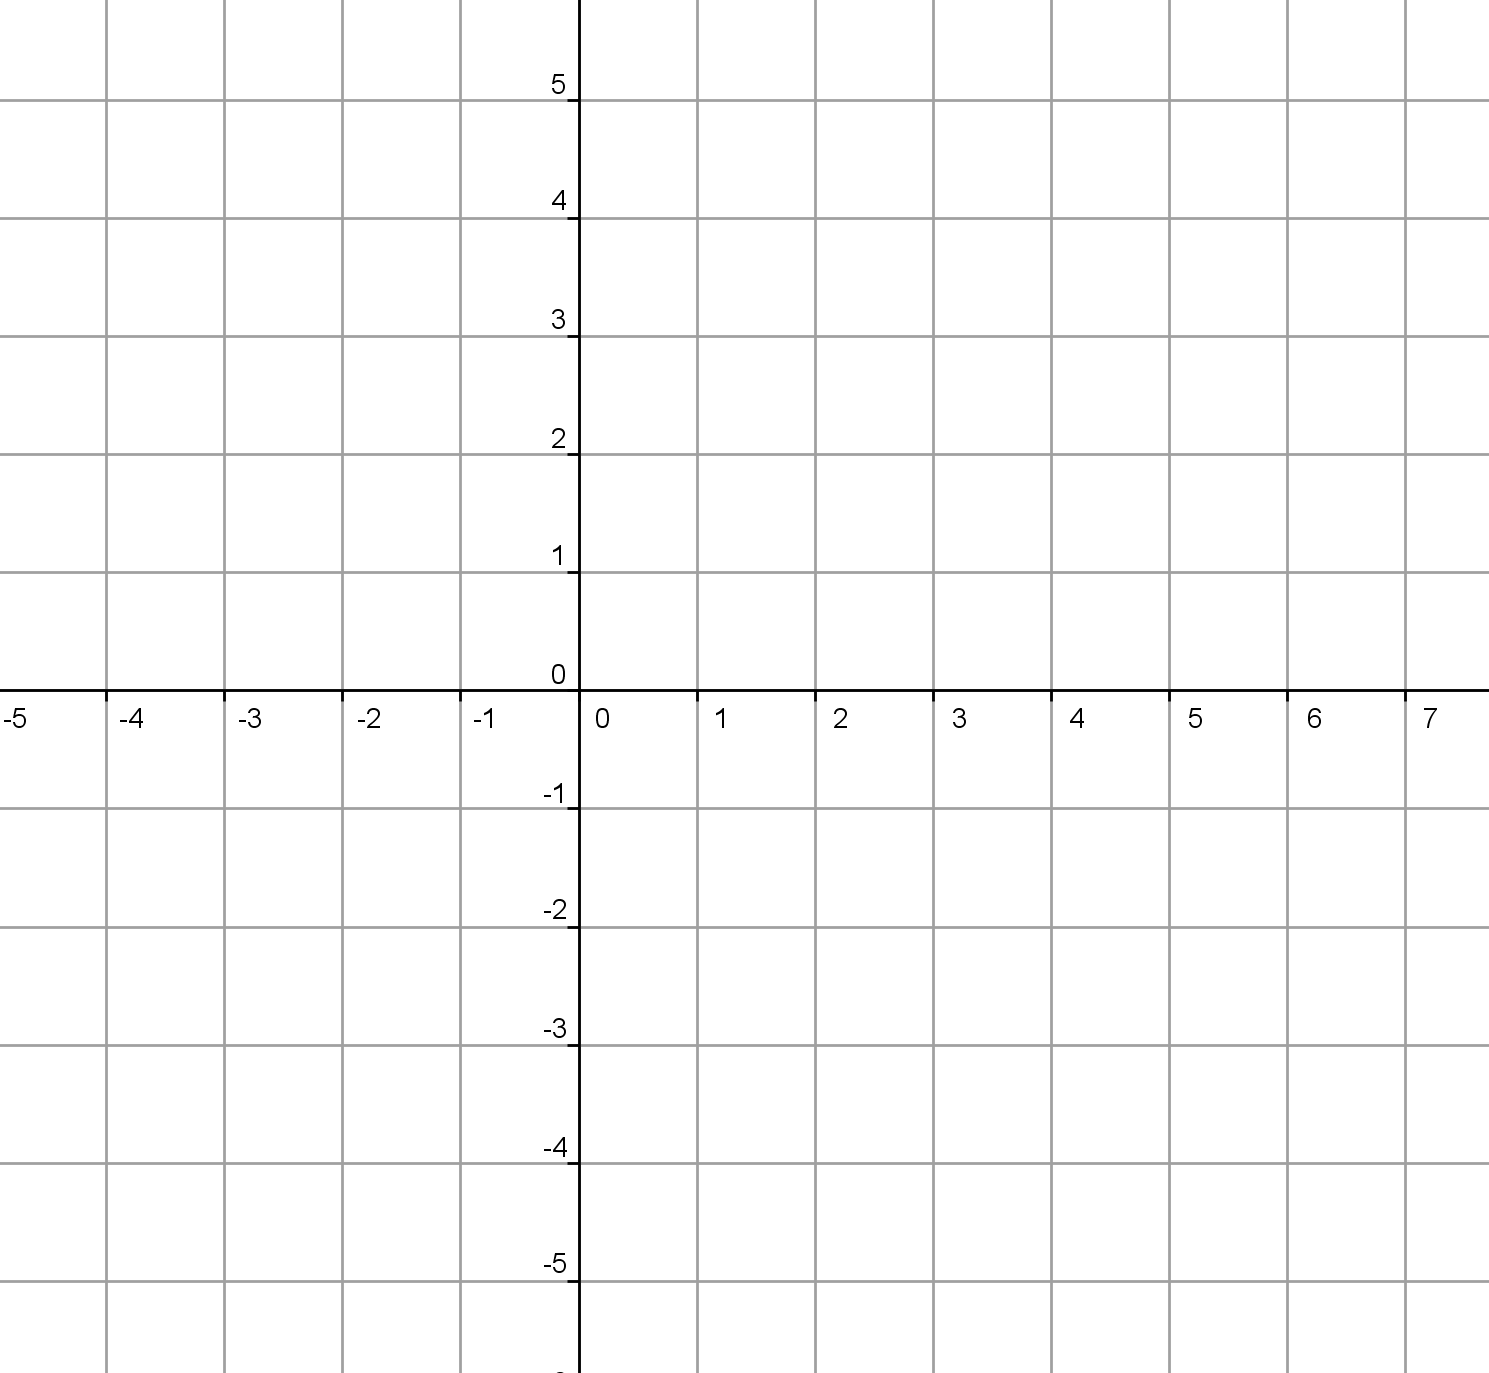
\includegraphics[width=7cm]{images/ex4.png} 
\end{minipage}
\end{tabular}

\bigskip

\ul{Exercice 5}: \textit{5 points}

Soit une fonction affine $k$.
Les points D(2;5) et E(-6;4) appartiennent �  sa repr�sentation graphique.

\begin{enumerate}
  \item Calculer le coefficient directeur de la fonction $k$.
  \item Calculer l'ordonn�e � l'origine de la fonction $k$.
  \item Donner l'expression alg�brique de la fonction $k$.
\end{enumerate}


\ldots \ldots \ldots \ldots \ldots \ldots \ldots \ldots \ldots \ldots \ldots
\ldots \ldots \ldots \ldots \ldots \ldots \ldots \ldots \ldots \ldots \ldots
\ldots \ldots \ldots \ldots \ldots \ldots \ldots \ldots \ldots \ldots \ldots
\ldots \ldots \ldots  

\ldots \ldots \ldots \ldots \ldots \ldots \ldots \ldots \ldots \ldots \ldots
\ldots \ldots \ldots \ldots \ldots \ldots \ldots \ldots \ldots \ldots \ldots
\ldots \ldots \ldots \ldots \ldots \ldots \ldots \ldots \ldots \ldots \ldots
\ldots \ldots \ldots  

\ldots \ldots \ldots \ldots \ldots \ldots \ldots \ldots \ldots \ldots \ldots
\ldots \ldots \ldots \ldots \ldots \ldots \ldots \ldots \ldots \ldots \ldots
\ldots \ldots \ldots \ldots \ldots \ldots \ldots \ldots \ldots \ldots \ldots
\ldots \ldots \ldots  

\ldots \ldots \ldots \ldots \ldots \ldots \ldots \ldots \ldots \ldots \ldots
\ldots \ldots \ldots \ldots \ldots \ldots \ldots \ldots \ldots \ldots \ldots
\ldots \ldots \ldots \ldots \ldots \ldots \ldots \ldots \ldots \ldots \ldots
\ldots \ldots \ldots  





\end{document}
